\begin{figure*}[!hbt]
    \caption{Approach overview}
    \centering
    \label{fig:approach_overview}
    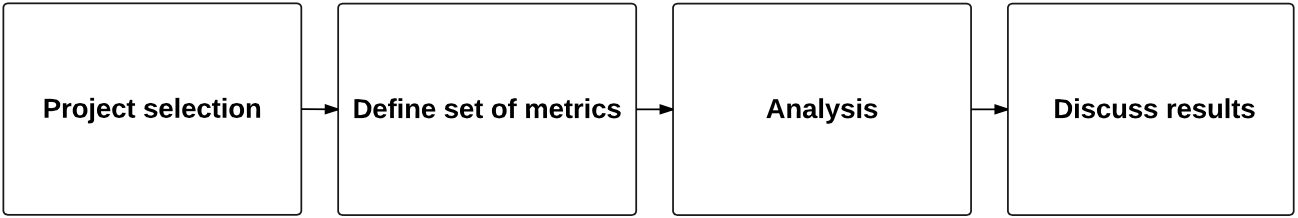
\includegraphics[width=1\textwidth]{figures/approach_overview}
 \end{figure*}


In this section we explain in details each one of the steps that we executed in our study. As shown in Fig \ref{fig:approach_overview} we first prepared all tags to run the source code analysis. Second we process all the tags in SonarQube. Third we extract the analyzed data from SonarQube and store it in our database. Fourth, we mine GitHub repositories to retrieve commit information and issues. Finally we process the data and run our analysis to answer the research questions.  \todo{create new approach figure}
 
\subsection{Create tags}

After selecting projects we had to find an automatic way to have all versions checked out, and ready for analysis. Instead of downloading each version separately, we devise a viable and more efficient technique. We cloned the latest release containing the \textit{\.git} folder in it. Then we write a script to checkout each tag based on the tags that git itself gives us by running \textit{`git log --tags --date-order --reverse --simplify-by-decoration --pretty=\%ai \%d'}. This command will return to us all the tags available in the repository ordered by date. Keeping the chronological order of the tags is important as our analysis in SonarQube has to be done in chronological order as well. 

The next process in our script check all the directories of the created tag searching for third-party libraries folders and remove them. We created a regular expression for this mean. 

The last process run when creating the tag is the addition of the sonar properties file. This file contains information about the created tag and is mandatory to run SonarQube analysis.


\subsection{Run SonarQube analysis}

\par
Each version of each application has been analyzed with a powerful source code analyzer tool named SonarQube. The resulting analysis of this tool contain metrics that are relevant to study evolution of software. 
\par
We also used this tool to identify anti-patterns that developers do in JavaScript. The results of this analysis is categorized in order of their severity. The possible classifications are `blocker', `critical', `major', `minor' and `info'.
\par
The default analysis process of SonarQube considers the current date as the date of the processed tag. This behavior does not allow us to observe the evolution between the different versions over time, as we run all analysis at once. To fix this problem, we set the desired date in a property file that is loaded in the beginning of each analysis. This file is generated automatically when we create the tags. 

In order to process 1065 tags, and to enforce that the chronological order will be maintained even in case of error we created a script to automate this process.
The script verifies if the tag was processing correctly or with error. Based on the result it decides if is necessary process again or to advance to the next tag. The total time to  process all tags with using this script was of 19 hours.

\subsection{Extract data from SonarQube}
\par After analyzing every tag in SonarQube we extract set of metrics that previous studies found proper for studying evolution of software projects. Metrics such as McCabe cyclomatic complexity, comment line density, duplicated lines and blocks, number of directories, statements and etc. Table  \ref{tab:metrics_definition} defines sets of metrics that we used in our analysis.

\par
Lehman suggests using the number of `modules' as the best way to measure the size of a large software system \cite{Lehman1997METRICS}. However, we decided to use the number of uncommented lines of code (`uncommented LOC') like the way Godfrey et al. \cite{Godfrey2000ICMS} did the evolution study on Linux Kernel. On the other hand we measure the comment lines and the ratio of comments to lines of codes, and based on that we can infer how much developers tend to put comments within their codes. We have to consider hidden corners that can mislead results, for example descriptive comments are totally different to the lines of codes that got commented because of refactoring or changes which considered as light-weight code smells in the code.

\par
We want to measure various aspects of the growth of these applications by having metrics. We also extract amount of duplications known as clones in terms of lines of codes, blocks and files. We would measure the cyclomatic complexity over time which the metric is calculated as following. Whenever the control flow of a function splits, the complexity counter gets incremented by one. Each function has a minimum complexity of 1. The control flow can split by conditional statements like if/else, switch case and so on. This metric is also known as also known as McCabe metric
We use the term `source file' to mean any file whose name ends with \textit{`.js'}.

\begin{figure*}[thb!]
	\caption{Lines of code evolution}
	\label{fig:lines_of_code}
	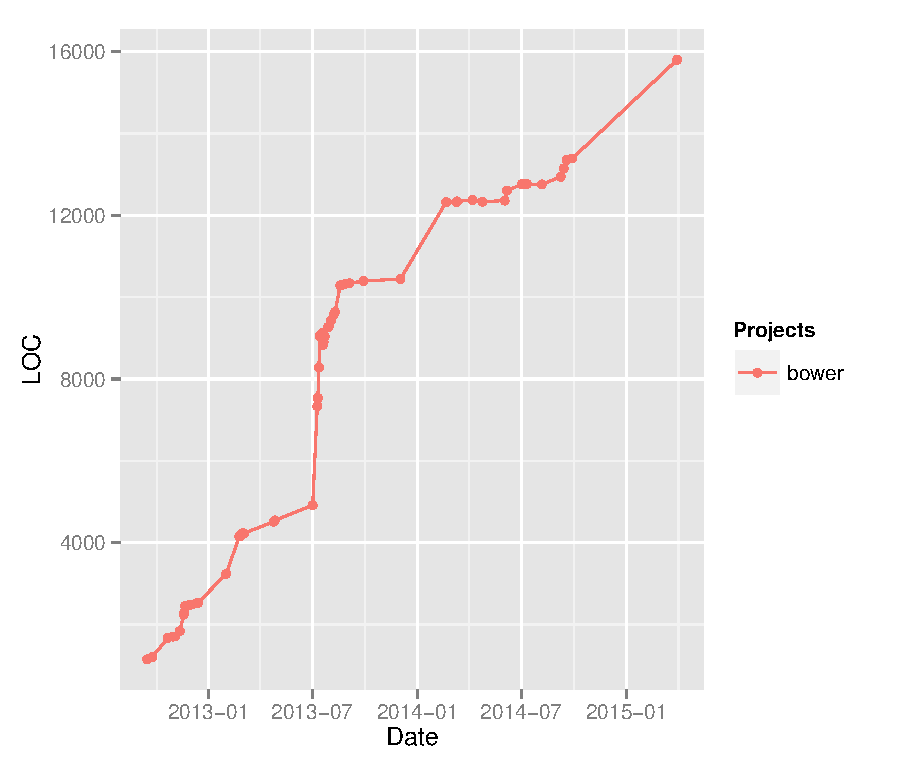
\includegraphics[width=90mm,scale=0.5]{figures/bower_loc}
	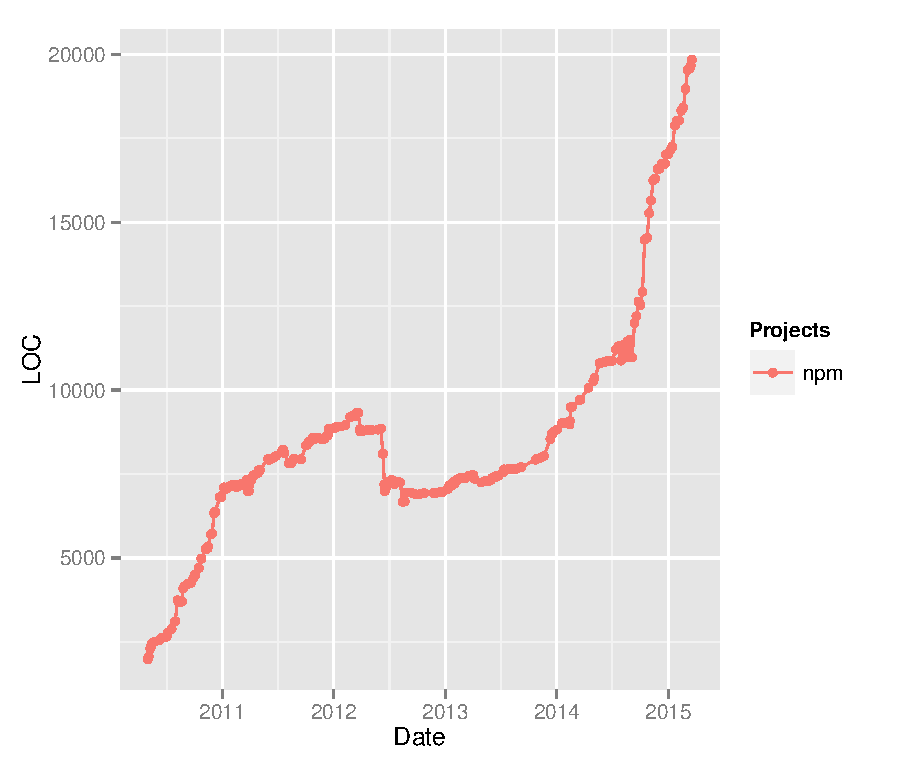
\includegraphics[width=90mm,scale=0.5]{figures/npm_loc}
	\centering
	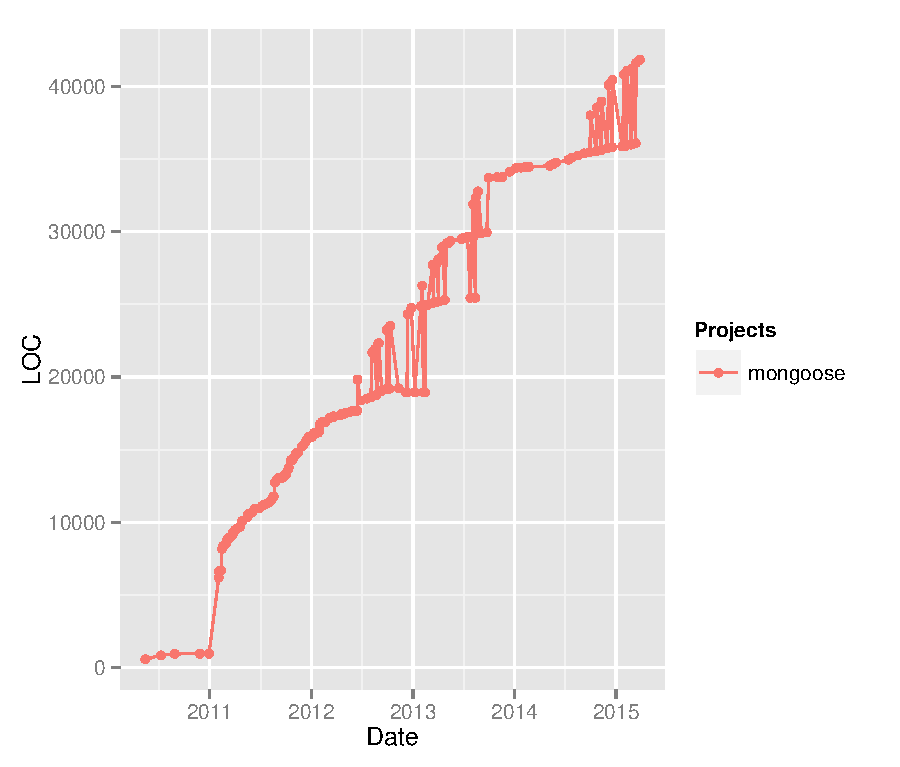
\includegraphics[width=90mm,scale=0.5]{figures/mongoose_loc}
\end{figure*}

In order to extract data from SonarQube we create a script to crawl through metrics comparison page of SonarQube to extract data. The data extracted from the web pages is stored in a CSV file and imported into the database later. At the beginning we tried to extract data from SonarQube public API but we found it immature at some points. We opted to use a crawler script instead of accessing SonarQube database directly because there is not a clear documentation of how SonarQube database schema is defined and, due to the high number of tags and projects that we are processing create queries for each one of them would be unfeasible. 

 \begin{table*}[!hbt]
    \begin{center}
        \caption{Selected metrics definition}
        \label{tab:metrics_definition}
        \begin{tabular}{c| l l }
            \toprule
            \textbf{Metric} & \textbf{Definition} \\ \midrule
            Lines of Code & The number of uncommented lines of code    \\
            Complexity      & McCabe complexity    \\
            Complexity/function & Average complexity by function. \\
            Complexity/file & Average complexity by file \\
            Comment lines  & Number of lines containing either comment or commented-out code. \\
            Comment Lines (\%)   & Density of comment lines = Comment lines / (Lines of code + Comment lines) * 100    \\
            Duplicated lines (\%)     & Density of duplication = Duplicated lines / Lines * 100    \\
            Duplicated blocks   & Number of duplicated blocks of lines    \\
            Directories   & Number of directories    \\
            Functions         & Number of functions    \\
            Statements        & Number of statements   \\
            Code Issues       & Number of issues with severity of blocker, critical, major and minor   \\
            Technical debt    & Number of days it takes to fix issues with respect to their severity    \\
            Technical debt ratio   & Division of SQALE Index by the estimation effort to re-develop your application from scratch.    \\
        \end{tabular}
    \end{center}
 \end{table*}

\subsection{Mine the source and issue tracker repositories}

There are at least two possible ways to extract commit information. One is by cloning the repository and then running git commands to extract the commits, and the other is using the API. We opted to extract the commits from the source code using the API. This API provides access to all public available data in any repository hosted at GitHub. Another important reason is that in our understanding is easier to create an automated process to extract this data using the API. 

We create a script that extract all commits from a given the repository name. This script stores the requested information in a \textit{JSON} format. Then we create a parser that retrieve data to put into create database for analysis purpose.

To extract the information of the issue tracker repository we apply the same approach. We created one script to request the information using the API and a second script to parse the file and store it in the database.

\subsection{Process the data}
After importing the metrics from SonarQube and mining the source and issue tracker repositories we need to process and transform this data to use it in our analysis. 

First, we make all the necessary transformations in the data extracted using the crawler script. As we get the data in the state that it appears to the user on a page, we need to convert and format dates to its specific type in the database. Then we need to do the same approach for numbers. Some of them were acquired as percentages and others was separated by commas. We run several \textit{P-SQL} scripts to complete this transformation.

Second, we link the extracted commits with each one of the tags using the commit date and the tag date. If the commit date is greater of tag release date and less than next tag of release date then the commit belongs to that tag. Third, we link the extracted issues with each one of the tags using the reported date and the tag date. If the reported date is greater  tag release date and less than the next tag release date then the issue belongs to that tag.